\documentclass[border=10pt]{standalone}

\usepackage{tikz}
\usepackage{tikzsymbols}
\usetikzlibrary{calc,patterns,shapes.geometric}

\def\centerarc[#1](#2)(#3:#4:#5){\draw[#1] ($(#2)+({#5*cos(#3)},{#5*sin(#3)})$) arc (#3:#4:#5);}

\begin{document}
	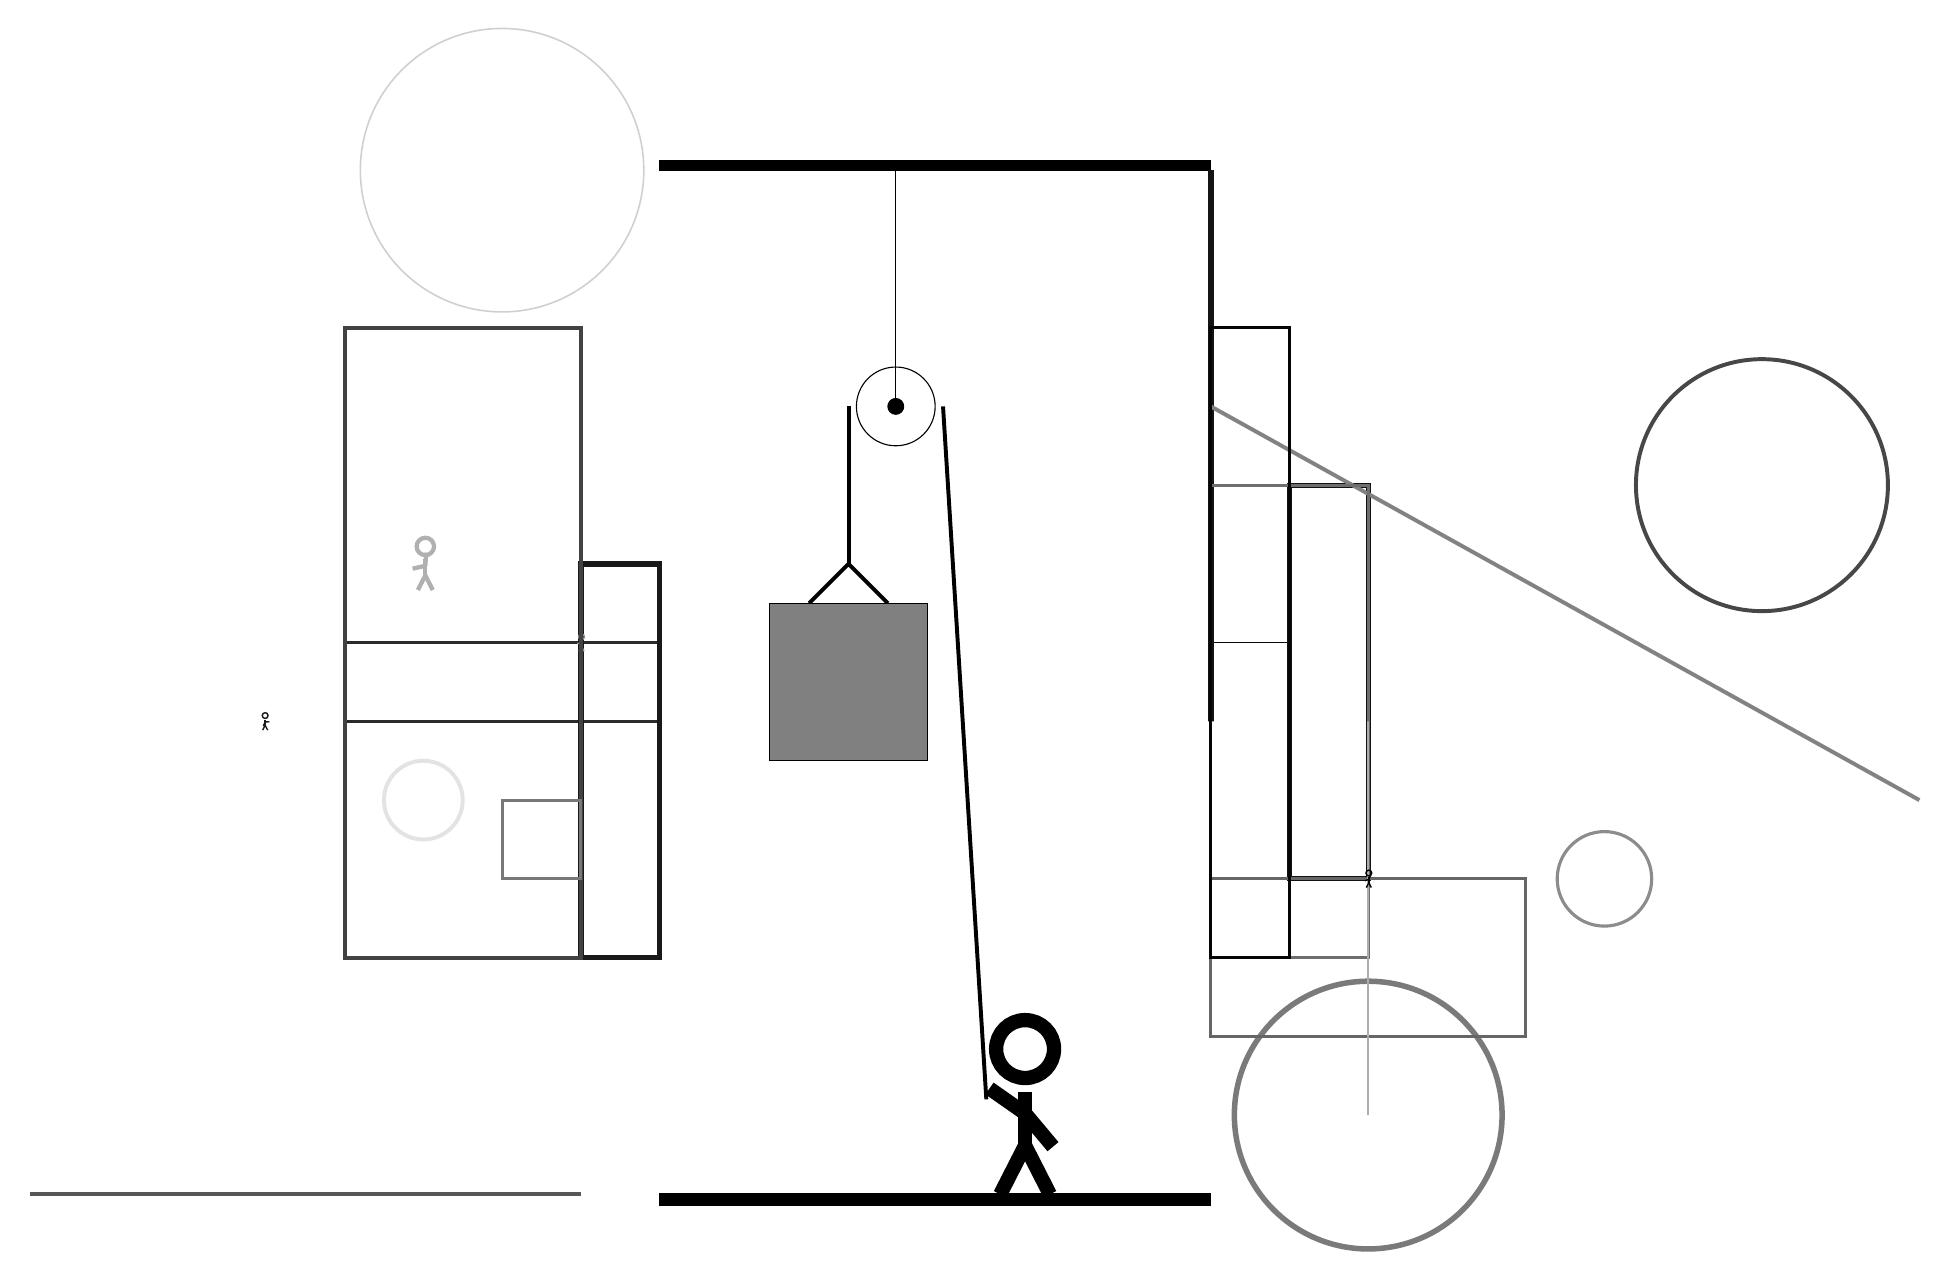
\begin{tikzpicture}
		%%%%% START %%%%%
		
		\draw[fill=black] (-2, 10) rectangle (5, 10.125);
		
		\draw[line width=0.2mm, color=black!96] (5, 4) rectangle (6, 8);
		
		\draw[line width=0.7mm, color=black!92] (5, 3) rectangle (5, 10);
		\draw[line width=0.6mm, color=black!93] (7, 1) rectangle (6, 6);
		\draw[line width=0.5mm, color=black!66](-3, -3) -- (-10, -3);
		
		\draw[line width=0.3mm, color=black!83] (-2, 3) rectangle (-6, 4);
		
		\draw [line width=0.2mm, color=black!19](-4, 10) circle (1.8);
		
		\draw[line width=0.7mm, color=black!90] (-2, 5) rectangle (-3, 0);
		\draw[line width=0.5mm, color=black!49](5, 7) -- (14, 2);
		\draw [line width=0.4mm, color=black!45](10, 1) circle (0.6);
		
		\draw [line width=0.7mm, color=black!52](7, -2) circle (1.7);
		\draw[line width=0.4mm, color=black!57] (5, 0) rectangle (7, 6);
		\node[line width=0.2mm, color=black!44] at (-3, 4) {\Strichmaxerl[1][3][86]};
		\draw[line width=0.4mm, color=black!60] (5, -1) rectangle (9, 1);
		
		\draw[line width=0.5mm, color=black!74] (-3, 8) rectangle (-6, 0);
		\draw[line width=0.2mm, color=black!32] (7, 3) rectangle (7, -2);
		\draw [line width=0.5mm, color=black!72](12, 6) circle (1.6);
		
		\node[line width=0.4mm, color=black!90] at (-7, 3) {\Strichmaxerl[1][66][4]};
		\draw[line width=0.4mm, color=black!53] (-4, 1) rectangle (-3, 2);
		\node[line width=0.3mm, color=black!31] at (-5, 5) {\Strichmaxerl[3][13][86]};
		\node[line width=0.2mm, color=black!98] at (7, 1) {\Strichmaxerl[1][17][68]};
		\draw [line width=0.5mm, color=black!11](-5, 2) circle (0.5);
		\draw[line width=0.4mm, color=black!98] (5, 0) rectangle (6, 8);
		
		
		\draw (1, 7) circle (0.5);
		\draw[fill=black] (1, 7) circle (0.1);
		\draw (1, 10) -- (1, 7);
		
		\draw[line width=0.5mm] (-0.1, 4.5) -- (0.4, 5.0) -- (0.9, 4.5);
		\draw[fill=black!50] (-0.6, 4.5) rectangle (1.4, 2.5);
		
		\draw[line width=0.5mm] (0.4, 7) -- (0.4, 5.0);
		\centerarc[line width=0.5mm](1, 7)(0:180:0.6);
		\draw[line width=0.5mm](1.6, 7) -- (2.15, -1.8);
		
		\node at (2.6, -1.9) {\Strichmaxerl[10][-35][-50]};
		
		\draw[fill=black] (-2, -3) rectangle (5, -3.15);
		
		%%%%% END %%%%%
	\end{tikzpicture}
\end{document}